\chapter{Can Quantum-Mechanical Description of Physical Reality Be Considered Complete?}
\label{chapter_2}

\authors{A. {\titleshape Einstein}, B. {\titleshape Podolsky}, N. {\titleshape Rosen}}

\begin{abstract} 
In a complete theory there is an element corresponding to each element of reality. A sufficient condition for the reality of a physical quantity is the possibility of predicting it with certainty, without disturbing the system. In quantum mechanics in the case of two physical quantities described by non-commuting operators, the knowledge of one precludes the knowledge of the other. Then either (1) the description of reality given by the wave function in quantum mechanics is not complete or (2) these two quantities cannot have simultaneous reality. Consideration of the problem of making predictions concerning a system on the basis of measurements made on another system that had previously interacted with it leads to the result that if (1) is false then (2) is also false. One is thus led to conclude that the description of reality as given by a wave function is not complete.
\end{abstract}

My name is Albert Einstein and I was a genius when I was alive. 
\begin{equation}
E = m c^2
\end{equation}

% Print figure caption on next page
\begin{FPfigure}
\centering
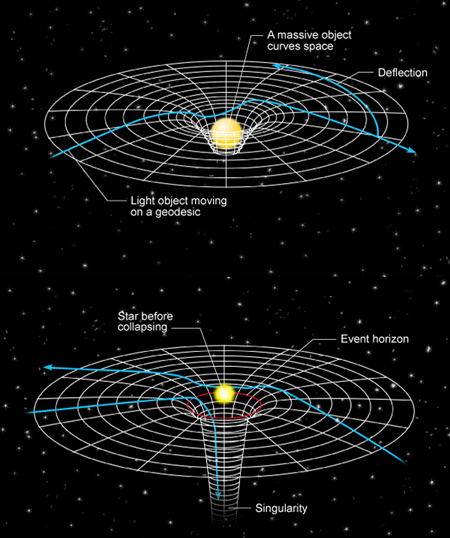
\includegraphics[width=\textwidth]{./chapter-1/figures/GR_picture.png}
\caption[A random figure about general relativity]{\textbf{Show caption of figure on the next page.}. A random figure about general relativity, not related to the rest of this thesis. (Top) In Einstein's general theory of relativity, gravity is nothing more than the curvature of spacetime. A massive object, such as the sun, causes a deformation of the spacetime grid, while another object such as a planet or a light beam follows the shortest path (a ``geodesic'') on this grid. To an observer, this looks like a deflection of the trajectory caused by gravity. (Bottom) A collapsing star can form a black hole so dense and massive that it creates a region of infinite curvature (a ``singularity'') so that --- inside the event horizon --- light cannot escape. Current research in gravitation is attempting to modify general relativity to account for such objects consistent with quantum theory.}
\end{FPfigure}